% Math Packages
\usepackage{amsmath, amsfonts, mathtools, amsthm,extarrows, amssymb,bbm} % unicode-math

% Programming Packages
\usepackage{pythonhighlight}

% Color
\definecolor{CustomColorChoice}{cmyk}{0,0.27,0.51,0.38,0}

% Citations
\usepackage{natbib}

\usepackage{hyperref}
\newcommand{\link}[2]{{\bfseries\color{CustomColorChoice!85}\href{#1}{#2}}}
 
% Figures
\usepackage{graphicx}
\graphicspath{{./figures/}}

% Congruent Modulo
\newcommand{\cmod}[3]{ #1 \text{ } \equiv \text{ } #2 \text{ } (\mathrm{mod} \ #3)}

% Contents
\usepackage{tocloft}

\renewcommand\contentsname{Summary of Contents}
\renewcommand\cfttoctitlefont{\Large\bfseries\sffamily}
\renewcommand\cftaftertoctitle{\hfill}

% Formatting
\usepackage[utf8]{inputenc}
\usepackage[T1]{fontenc}

% Tables
\usepackage{booktabs, tabularx}

% Shortcuts (N, R, Z, etc.)
\newcommand\N{\ensuremath{\mathbb{N}}}
\newcommand\Prob{\ensuremath{\mathbb{P}}}
\newcommand\R{\ensuremath{\mathbb{R}}}
\newcommand\Z{\ensuremath{\mathbb{Z}}}
\renewcommand\O{\ensuremath{\emptyset}}
\newcommand\Q{\ensuremath{\mathbb{Q}}}
\newcommand\C{\ensuremath{\mathbb{C}}}
\newcommand\fpa{\tilde{f}_{\texttt{FP}}}
\newcommand\ipa{\tilde{f}_{\texttt{IP}}}
\newcommand\mA{\mathbf{A}}
\newcommand\mB{\mathbf{B}}
\newcommand\mV{\mathbf{V}}
\newcommand\mC{\mathbf{C}}

% Floor and Cieling
\newcommand{\floor}[1]{\left\lfloor #1 \right\rfloor}
\newcommand{\ceil}[1]{\left\lceil #1 \right\rceil}

% Title Formatting
\titleformat*{\section}{\Large\bfseries\sffamily}
\titleformat*{\subsection}{\large\bfseries\sffamily}
\titleformat*{\subsubsection}{\itshape\sffamily}

% Horizontal Line
\newcommand{\NewLine}{\vspace{0.5pc}}
\newcommand{\LineBreak}{\vspace{0.5pc} \noindent \textcolor{CustomColorChoice}{\makebox[\linewidth]{\rule{\linewidth}{0.4pt}}} \vspace{0.5pc}}

% Example Box Formatting
\usepackage[most]{tcolorbox}

\tcbuselibrary{theorems}
\newtcbtheorem[]{ex}{\textbf{Example}}{
  	breakable,
    colback=CustomColorChoice!5,
    colframe=CustomColorChoice!85,
    fonttitle=\sffamily\color{White}
  }{def}

 % Theorem and Proof Formatting
\usepackage{thmtools}

\declaretheoremstyle[
    headfont=\bfseries\sffamily\color{CustomColorChoice!85},
    bodyfont=\normalfont,
    mdframed={
        linewidth=2pt,
        usetwoside=false,
        rightline=false, topline=false, bottomline=false,
        linecolor=CustomColorChoice!85, backgroundcolor=CustomColorChoice!5,
    }
]{defnbox}

\declaretheoremstyle[
    headfont=\bfseries\sffamily\color{Black},
    bodyfont=\normalfont,
    mdframed={
        linewidth=2pt,
        rightline=false, topline=false, bottomline=false,
        linecolor=CustomColorChoice!85, backgroundcolor=white,
    }
]{thmbox}


\declaretheoremstyle[
    headfont=\bfseries\sffamily\color{Black},
    bodyfont=\normalfont,
    mdframed={
        linewidth=2pt,
        rightline=false, topline=false, bottomline=false,
        linecolor=CustomColorChoice!15, backgroundcolor=white,
    }
]{marginbox}

\declaretheoremstyle[
    headfont=\bfseries\sffamily\color{Black},
    bodyfont=\normalfont,
    mdframed={
        linewidth=2pt,
        rightline=false, topline=false, bottomline=false,
        linecolor=CustomColorChoice!85, backgroundcolor=white,
    }
]{rmkbox}

\declaretheoremstyle[
    headfont=\bfseries\sffamily\color{Black},
    bodyfont=\normalfont,
    numbered=no,
    mdframed={
        linewidth=2pt,
        rightline=false, topline=false, bottomline=false,
        linecolor=white, backgroundcolor=white,
    }
]{corbox}

\declaretheoremstyle[
    headfont=\bfseries\sffamily\color{CustomColorChoice!85},
    bodyfont=\normalfont,
    numbered=no,
    mdframed={
        linewidth=2pt,
        rightline=false, topline=false, bottomline=false,
        linecolor=white, backgroundcolor=white,
    },
    qed=\qedsymbol
]{proofbox}

 \declaretheorem[style=thmbox, numbered=yes, name=Lemma]{lem}
 \declaretheorem[style=thmbox, numbered=yes, name=Theorem]{thm}
  \declaretheorem[style=thmbox, numbered=yes, name=Proposition]{prop}
  \declaretheorem[style=thmbox, numbered=no, name=Conjecture]{conj}
 \declaretheorem[style=rmkbox, numbered=no, name=Note]{note}
 \declaretheorem[style=rmkbox, numbered=no, name=Remark]{rmk}
 \declaretheorem[style=corbox, numbered=no, name=Corollary]{cor}
  \declaretheorem[style=corbox, numbered=no, name=Derivation]{derivation}
 \declaretheorem[style=defnbox, numbered=no, name=Definition]{defn}
 \declaretheorem[style=proofbox, numbered=no, name=Proof]{replacementproof}

 \renewenvironment{proof}[1][\proofname]{\vspace{-10pt}\begin{replacementproof}}{\end{replacementproof}}

% Title Page
\makeatletter
\renewcommand{\maketitlepage}{
    \cleardoublepage{
        \begin{fullwidth}
        
        \fontsize{10}{14}\selectfont\par\noindent{\textbf{Semester}: Fall 2022}
        \fontsize{10}{14}\selectfont\par\noindent{\textbf{Instructor}: Lessard, Jean-Philippe}

        \vspace{2pc}
        
        \fontsize{36}{40}\selectfont\par\noindent{Numerical Analysis}
        
        \begin{center}
        
        \vspace{3pc}
        
        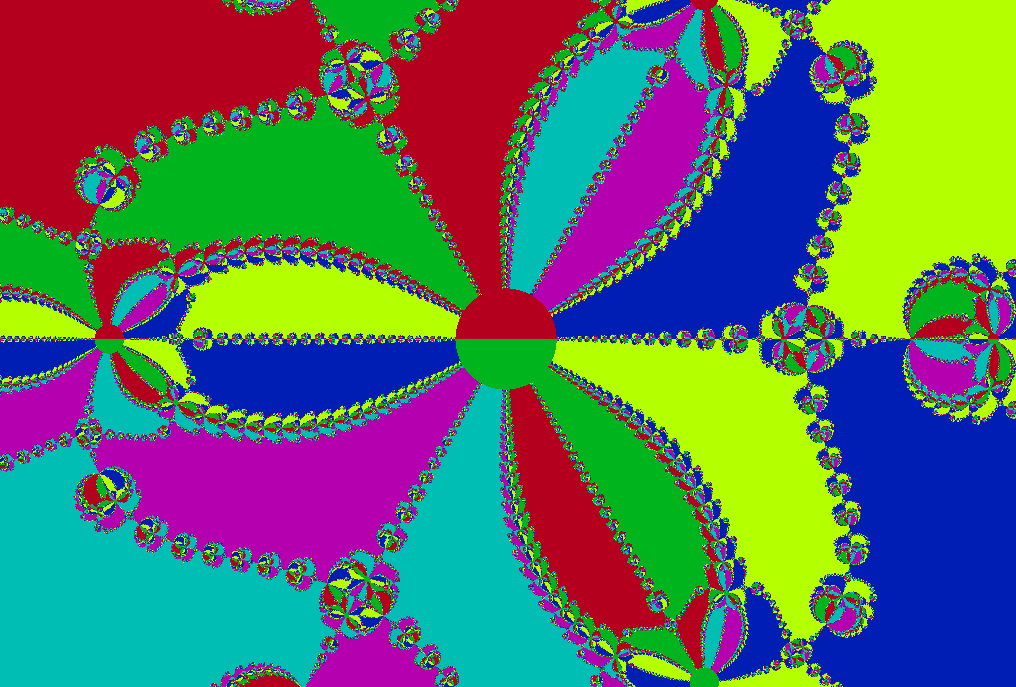
\includegraphics[width=\linewidth]{figures/title.png}
        \end{center}
        
        \vfill
        
        \fontsize{10}{14}\selectfont\par\noindent\thanklesspublisher{\textbf{Course Content.}  Error analysis. Numerical solutions of equations by iteration. Interpolation. Numerical differentiation and integration. Introduction to numerical solutions of differential equations.}
        \end{fullwidth}
    }
    \thispagestyle{empty}
    \clearpage
}
\makeatother

% Pseudocode
\usepackage{xcolor,amsmath}
\usepackage[linesnumbered,ruled,vlined]{algorithm2e}
\DontPrintSemicolon

\renewcommand{\KwSty}[1]{\textnormal{\textcolor{blue!90!black}{\ttfamily\bfseries #1}}\unskip}
\renewcommand{\ArgSty}[1]{\textnormal{\ttfamily #1}\unskip}
\SetKwComment{Comment}{\color{green!50!black}// }{}
\renewcommand{\CommentSty}[1]{\textnormal{\ttfamily\color{green!50!black}#1}\unskip}
\newcommand{\assign}{\leftarrow}
\newcommand{\var}{\texttt}
\newcommand{\FuncCall}[2]{\texttt{\bfseries #1(#2)}}
\SetKwProg{Function}{function}{}{}
\renewcommand{\ProgSty}[1]{\texttt{\bfseries #1}}



% C Code Formatting
\definecolor{mGreen}{rgb}{0,0.6,0}
\definecolor{mGray}{rgb}{0.5,0.5,0.5}
\definecolor{mPurple}{rgb}{0.58,0,0.82}
\definecolor{backgroundColour}{rgb}{0.95,0.95,0.92}

\lstdefinestyle{ExCStyle}{
    backgroundcolor=\color{CustomColorChoice!5},   
    commentstyle=\color{CustomColorChoice!50},
    keywordstyle=\bfseries\color{CustomColorChoice},
    numberstyle=\tiny\color{mGray},
    stringstyle=\color{mPurple},
    basicstyle=\small\ttfamily,
    breakatwhitespace=false,         
    breaklines=true,                 
    captionpos=b,                    
    keepspaces=true,
    numbers=none,            
    showspaces=false,                
    showstringspaces=false,
    showtabs=false,                  
    tabsize=2,
    language=Matlab
}